
\chapter{Pretty Printing}

Super-languages deal with a great deal of structured data. How is
the information to be managed? Model developers need a way of interacting
with the information in a flexible way. They should be able to look
at the data in a variety of ways, slicing it up and presenting it
as appropriate.

One approach to presenting model data in a flexible way is to use
an extensible pretty-printer. A pretty-printer is a system that can
be used to print out data in a convenient form; it provides hooks
to change the appearance of data items and also provides a means of
controlling the layout of large quantities of data. This chapter shows
how a pretty-printer can be modelled and implemented as an execution
engine that runs the models. It is an example of how XMF can be used
to develop a language engine. The pretty-printer language has no concrete
syntax, however it is still a language and has an engine that executes
it. The super-language features of XMF make it idea for defining a
pretty-printer language and its execution engine.


\section{Example Printing}

Consider a database of bank records. Each record describes a bank
customer in terms of their name, age and the unique account identifiers.
If the database is printed out without any attempt at layout then
the following might be the result:

\begin{lstlisting}
DataBase[records = Seq{Record[accounts = Seq{A101,B204,
A108},age= 22,name = Fred Jones],Record[accounts = 
Seq{C202},age = 32,name = Sally Brown],Record[accounts = 
Seq{A102,B222},age = 24,name = Edward Clark]}]
\end{lstlisting}Obviously no attempt has been made at structuring the information;
newlines occur at arbitrary points in the data where the right-hand
edge of the output window (or \textit{page}) is reached. The following
are significant factors in controlling the presentation of data:

\begin{itemize}
\item The type of an element determines how it should be presented. For
example, an atomic data item such as a string or a number is just
printed out as is. An object contains slots and the slot values are
possibly large elements in themselves. A basic object might be displayed
as a sequence of slots where there are many choices governing the
layout of the slots. Particular types of object might be displayed
in specific ways; for example, internal features of an object may
be considered as hidden and not printed out. Other types of element
that require specific display include tables, collections and vectors.
\item The width of the page is an important factor when displaying elements.
Often there may be a choice regarding how an element is to be laid
out on the page, for example an object may list its slots one after
the other on the same line or list the slots one above the other on
different lines. The width of the page can be used in deciding amongst
the alternatives.
\item Independent of the width of the page, is the maximum width of output
on any given line. Call this the ribbon width; it differs from the
page width because it dones not take into consideration leading whitespace
on a line. The ribbon width can be used to decide amongst alternative
layout strategies.
\item Complex data is usually deeply nested, i.e. one element contains another,
and that contains more data etc. Sometimes a broad picture of the
data is required; other times it is necessary to drill deeply into
an element. 
\end{itemize}
Using the example data given above, the following shows a borad view
with a wide page width and ribbon:

\begin{lstlisting}
DataBase[records = Seq{
                     Record[accounts = ...,age = 22,name = Fred Jones],
                     Record[accounts = ...,age = 32,name = Sally Brown],
                     Record[accounts = ...,age = 24,name = Edward Clark]}]
\end{lstlisting}The ... shows that the level of nesting limit has been reached. If
the level of nesting is decreased by 1 then the display would show
that the database had 3 records, but not show the records themselves:

\begin{lstlisting}
DataBase[records = Seq{...,...,...}]
\end{lstlisting}Alternatively, consider a short ribbon width and a deep nesting:

\begin{lstlisting}
DataBase[records = Seq{
                     Record[
                       accounts =
                         Seq{A101,B204,A108}
                       age = 22,
                       name = Fred Jones],
                     Record[
                       accounts = Seq{C202}
                       age = 32,
                       name = Sally Brown],
                     Record[
                       accounts = Seq{A102,B222}
                       age = 24,
                       name = Edward Clark]}]
\end{lstlisting}Finally taking this to its limit:

\begin{lstlisting}
DataBase[
  records =
    Seq{
      Record[
        accounts =
          Seq{
            A101,
            B204,
            A108}
        age =
          22,
        name =
          Fred Jones],
      Record[
        accounts =
          Seq{C202}
        age =
          32,
        name =
          Sally Brown],
      Record[
        accounts =
          Seq{
            A102,
            B222}
        age =
          24,
        name =
          Edward Clark]}]
\end{lstlisting}
\section{A Document Model}

%
\begin{figure}
\begin{center}

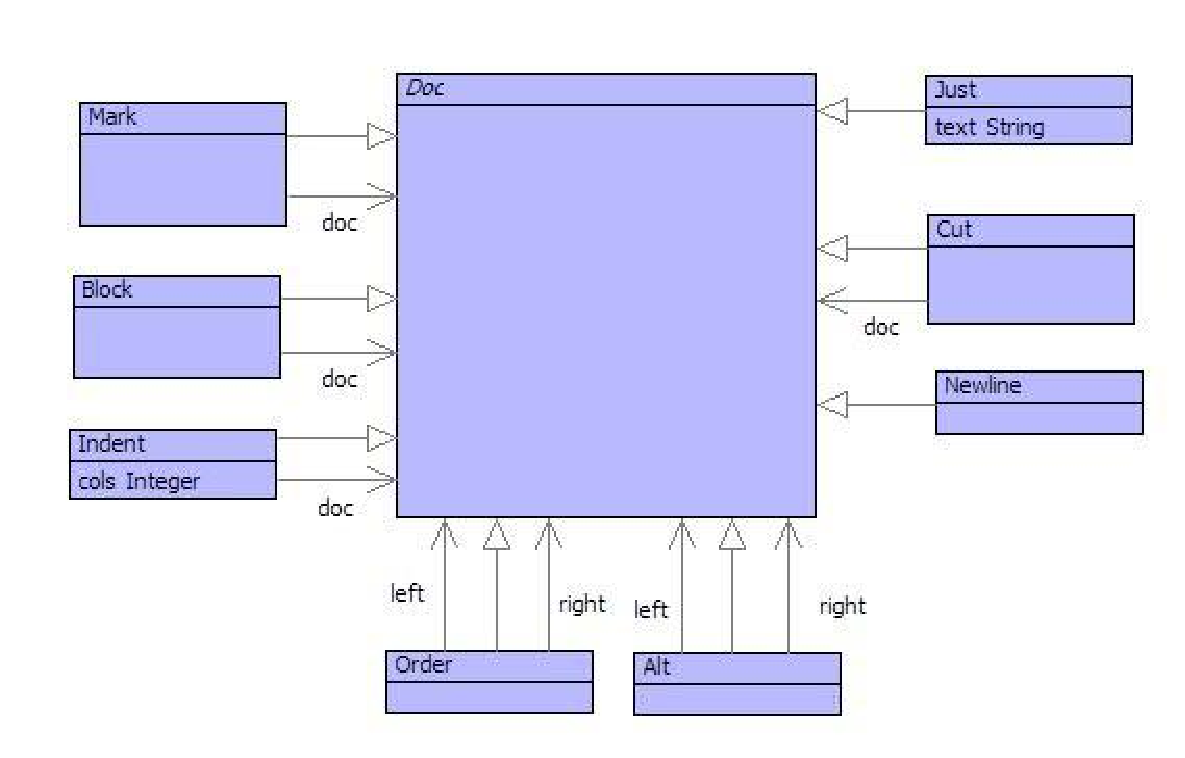
\includegraphics[width=12cm]{Programming/PrettyPrint/Images/Docs.pdf}
\caption{A Document Model\label{fig:A-Document-Model}}

\end{center}
\end{figure}


Pretty printing can be achieved by writing an output operation for
each new model element. In the example above, the database and record
classes would each define an output operation. The output operations
need to keep track of the page and ribbon widths, and also deal with
manging options for output. 

The general output machinery is more or less the same for each new
class; just the details of what is being printed differs from class
to class. Therefore it makes sense to abstract the machinery into
a general model of documents. 

A document consists of output directives including the text to be
printed. A mapping translates instances of classes to the document
model. Therefore, the machinery for pretty-printing is defined once
in the document model and domain models are not polluted with details
of printing.

The document model is shown in figure \ref{fig:A-Document-Model}.
The rest of this section describes the classes in the document model
and shows how they affect the output when printed prettily.

A document Just(t) represents just the text t. When it is printed
with a page and ribbon width of 80, the text is displayed:

\begin{lstlisting}
XMF> Just("some text").pprint(80,80);
some text
\end{lstlisting}By itself, Just does not appear to do anything; however, as described
later, Just may cause an alternative formatting to be chosen because
the text does not fit onto the current line or the current ribbon.

Several documents can be joined together using Order. Viewing the
pretty printer as sending text to an output ribbon, Order(d1,d2) just
causes the output from d1 to be printed to the ribbon followed by
the output from d2:

\begin{lstlisting}
XMF> Order(Just("some text"),
       Order(Just(" more text"),
             Just(" the end."))).pprint(80,80);
some text more text the end.
\end{lstlisting}Newline can be used to insert breaks into the output:

\begin{lstlisting}
XMF> Order(Just("some text"),
       Order(Newline(),
         Order(Just("more text"),
           Order(Newline(),
             Just("the end."))))).pprint(80,80);
some text
more text
the end.
\end{lstlisting}Indentation is important in output, it is often used to represent
ownership or containment. For example, collections own their elements
and objects own their slots. The display of the elements and slots
can be indented in order to represent ownership.

The engine that prints a document maintains a context including the
current level of indentation. Each time a new line is printed, the
engine automatically tabs to the current indent by adding spaces to
the output ribbon. The value of the current indent can be increased
by a given value using the class Indent:

\begin{lstlisting}
XMF> Order(Just("some text"),
      Indent(2,
        Order(Newline(),         
          Order(Just("then more text"),
            Indent(2,
              Order(Newline(),
                Just("the end."))))))).pprint(80,80);
some text
  then more text
    the end.
\end{lstlisting}The current level of indentation can be set using the class Block.
The document Block(d) uses the position on the current line as the
level of indentation for processing d. Once d has been processes,
the level of indentation reverts back:

\begin{lstlisting}
XMF> Order(Just("some text"),       
       Order(
         Block(
           Order(Newline(),
             Just("more text"))),
         Indent(2,
           Order(Newline(),
            Just("the end."))))).pprint(80,80);
some text
         more text
  the end.
\end{lstlisting}The arguments to the pprint operation are the page width and ribbon
width respectively. The docment classes described so far provide a
fixed output format: the values of page and ribbon width make no difference
to the output. As described earlier, it is desirable to be able to
print an element in different formats depending on the context: a
wide page width will allow an object to list its slots on the same
line ehwreas a narrow page width forces the slots to be listed one
above the other. 

The document Alt(d1,d2) defines two alternative layouts: d1 and d2.
When pretty printing the document Alt(d1,d2), the printer first tries
d1, if it finds that any of the output of d1 exceeds the line or ribbon
width then the printer discards the output from d1 and proceeds with
d2. Consider the following operations:

\begin{lstlisting}
@Operation line(.ss:Seq(String)):Doc
  ss->tail->iterate(s d = Just(ss->head) | Order(d,Just(" " + s)))
end
  
@Operation stack(.ss:seq(string)):Doc
  ss->tail->iterate(s d = Just(ss->head) | Order(d,Order(Newline(),Just(s))))
end
\end{lstlisting}The operation line transforms a sequence of strings into an ordered
document. The operation stack transforms a sequence of strings into
a document that displays the strings one above the other. The following
code shows two uses of the same document, the first prints on a page
width of 80 with a ribbon width of 80 and the second on the same page
with a ribbon width of 10. In the first case the text can fit on the
same line. In the second case the text cannot fit onto a ribbon with
of 10 and therefore the second option is used:

\begin{lstlisting}
XMF> let strings = Seq{"some text","more text","end."}
     in Alt(line(strings),stack(strings)).pprint(80,80)
     end;
some text more text end.
XMF> let strings = Seq{"some text","more text","end."}
     in Alt(line(strings),stack(strings)).pprint(80,10)
     end;
some text
more text
end.
\end{lstlisting}
\section{A Pretty Printing Machine}

%
\begin{figure}
\begin{center}

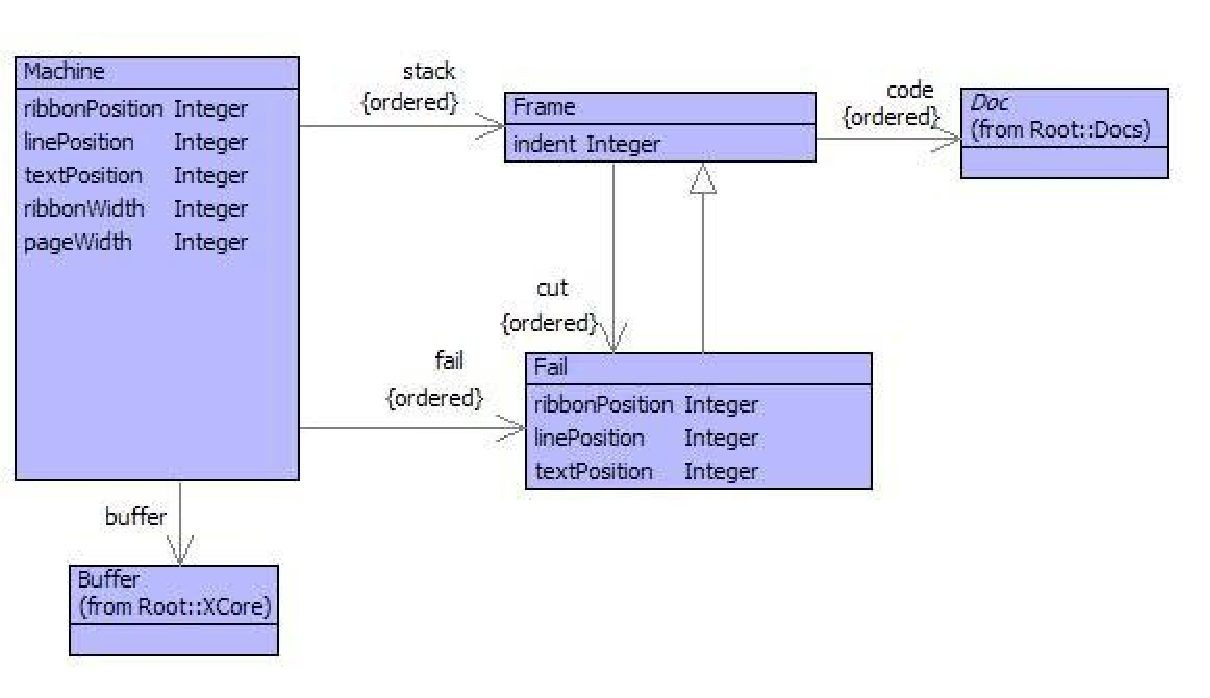
\includegraphics[width=12cm]{Programming/PrettyPrint/Images/Engine.pdf}

\caption{The Pretty Print Engine\label{fig:The-Pretty-Print-Engine}}

\end{center}
\end{figure}


A document is pretty-printed by a pretty-printing machine. The machine
\textit{runs} the document and the state of the machine includes the
page and ribbon width and the current text position on the page. The
machine model is shown in figure \ref{fig:The-Pretty-Print-Engine},
the rest of this section describes how the machine works.

A pretty-printer is an instance of the class Machine. The state of
a machine consists of the following:

\begin{itemize}
\item ribbonPosition is the next output position on the current line ignoring
any leading indentation;
\item linePosition is the next output position on the current line;
\item textPosition is the next output position on the page;
\item ribbonWidth is the maximum number of characters on a line ignoring
any leading indentation;
\item pageWidth is the maximum number of character on a line;
\item a buffer containing the output (next buffer position is given by textPosition);
\item stack is a sequence of frames;
\item fail is a sequence of fail frames.
\end{itemize}
The stack contains a sequence of frames. Each frame contains a sequence
of documents to be printed along with the indentation used for their
output. Frames allow the indentiation in a document to change: when
the machine runs it prints out all the documents in the frame at the
head of the stack, when those documents are completed then the machine
pops the stack and continues with the next frame. If a document wants
to change the indentation for a given document then it pushes a new
frame at the head of the stack.

A machine has a sequence of fail frames. When a Just(t) document is
executed at the head of the stack, if the text t cannot be printed
out in the current page and ribbon width then the machine attempts
to \textit{fail}. Failure involves returning to a choice point defined
by an instance of the class Fail containing a saved machine state.
To fail, the machine resets all the saved state in the Fail instance
and then pops the fail stack.

\begin{lstlisting}
@Operation run()
  @While not stack->isEmpty do
    if stack->head.code()->isEmpty
    then self.stack := stack->tail
    else
      let frame = stack->head then
          instr = frame.code()->head 
      in stack->head.setCode(frame.code()->tail);
         @Case instr of
           Just(text) do
             if self.canPrint(text) or fail->isEmpty
             then self.write(text)
             else self.fail() 
             end
           end
           Order(left,right) do
             frame.setCode(Seq{left,right} + frame.code()) 
           end
           Indent(cols,doc) do
             self.pushFrame(frame.indent() + cols,frame.cut(),Seq{doc})
           end
           Block(doc) do
             self.pushFrame(linePosition,frame.cut(),Seq{doc})
           end
           Cut(doc) do 
             self.fail := frame.cut()
           end
           Mark(doc) do
             self.pushFrame(frame.indent(),fail,Seq{doc})
           end
           NewLine() do
             self.newline()
           end
           Alt(left,right) do
             frame.setCode(Seq{left | frame.code()});
             self.pushFail(Seq{right | frame.code()})
           end
         end
      end
    end
  end
end
\end{lstlisting}%
\begin{figure}
\begin{center}
\begin{tabular}{|c|c|}
\hline
\begin{minipage}{2in}
\begin{lstlisting}

(1)Machine[80,50,0,0,0,
  [],
  Seq{Frame[0,
    code = Seq{
      some text; 
       more text; 
       the end.},
    cut = Seq{}
    ]},
  Seq{}]

\end{lstlisting}
\end{minipage}
&
\begin{minipage}{2in}
\begin{lstlisting}
(2)Machine[80,50,0,0,0,
  [],
  Seq{Frame[0,
    code = Seq{
      some text, 
       more text; 
       the end.},
    cut = Seq{}
    ]},
  Seq{}]
\end{lstlisting}
\end{minipage}
\\\hline
\begin{minipage}{2in}
\begin{lstlisting}

(3)Machine[80,50,9,9,9,
  [some text],
  Seq{Frame[0,
    code = Seq{
      more text; 
      the end.},
    cut = Seq{}
    ]},
  Seq{}]

\end{lstlisting}
\end{minipage}
&
\begin{minipage}{2in}
\begin{lstlisting}
(4)Machine[80,50,9,9,9,
  [some text],
  Seq{Frame[0,
    code = Seq{
      more text, 
      the end.},
    cut = Seq{}
    ]},
  Seq{}]
\end{lstlisting}
\end{minipage}
\\\hline
\begin{minipage}{2.3in}
\begin{lstlisting}

(5)Machine[80,50,19,19,19,
  [some text more text],
  Seq{Frame[0,
    code = Seq{ the end.},
    cut = Seq{}
    ]},
  Seq{}]

\end{lstlisting}
\end{minipage}
&
\begin{minipage}{2.7in}
\begin{lstlisting}
(6)Machine[80,50,28,28,28,
  [some text more text the end.],
  Seq{Frame[0,
    code = Seq{},
    cut = Seq{}
    ]},
  Seq{}]
\end{lstlisting}
\end{minipage}
\\\hline
\end{tabular}

\caption{Execution of Ordered Text\label{fig:Execution-of-Ordered}}

\end{center}
\end{figure}


Figure \ref{fig:Execution-of-Ordered} shows the steps taken by the
machine when it processes a document consisting of 3 ordered strings.
The machine is printed (using the pretty printer) as Machine{[} followed
by the page width, ribbon width, text position, line position and
ribbon position. The contents of the output buffer is on the following
line inside {[} and ]. The stack frames are printed next, followed
by the fail frames. Each frame is printed as Frame{[} followed by
the value used for indentation. The code and cut values follow on
the next lines. To save space, Order(d1.d2) is printed as d1;d2.

State (1) is the starting state. State (2) shows that the ordered
document at the head of the stack is processed first. State (3) has
output the first string, notice how the values of the positions in
the machine state have been updated. State (4) handles the ordered
document at the head of the stack. States (5) and (6) output the second
and third strings. State (6) is a terminal state because there is
a single frame with empty code.

Consider pretty-printing the following:

\begin{lstlisting}
Order(Just("some text"),
  Order(
    Block(
      Order(Newline(),
        Just("more text"))),
    Indent(2,
      Order(Newline(),
        Just("the end.")))))
\end{lstlisting}The machine starts in the following state:

\begin{lstlisting}
Machine[80,50,0,0,0,
  [],
  Seq{
    Frame[0,
      code = Seq{
               some text;
               ...;
               Indent[2
                 ...;
                 ...]},
      cut = Seq{}
      ]},
  Seq{}]
\end{lstlisting}The machine prints some text on the output and then encounters the
block:

\begin{lstlisting}
Machine[80,50,9,9,9,
  [some text],
  Seq{
    Frame[0,
      code = Seq{
               Block[
                 doc = 
                   ...;
                   ...];
               Indent[2
                 ...;
                 ...]},
      cut = Seq{}
      ]},
  Seq{}]
\end{lstlisting}A new frame is pushed that records the current indent position:

\begin{lstlisting}
Machine[80,50,9,9,9,
  [some text],
  Seq{
    Frame[9,
      code = Seq{
               Newline[];
               more text},
      cut = Seq{}
      ],
    Frame[0,
      code = Seq{
               Indent[2
                 ...;
                 ...]},
      cut = Seq{}
      ]},
  Seq{}]
\end{lstlisting}The newline and more text is printed with respect to the frame at
the head of the stack:

\begin{lstlisting}
Machine[80,50,28,18,9,
  [some text
         more text],
  Seq{
    Frame[9,
      code = Seq{},
      cut = Seq{}
      ],
    Frame[0,
      code = Seq{
               Indent[2
                 ...;
                 ...]},
      cut = Seq{}
      ]},
  Seq{}]
\end{lstlisting}The empty frame is popped, processing resumes with the Indent causing
a new frame to be pushed with an indent of 2:

\begin{lstlisting}
Machine[80,50,28,18,9,
  [some text
         more text],
  Seq{
    Frame[2,
      code = Seq{
               Newline[];
               the end.},
      cut = Seq{}
      ],
    Frame[0,
      code = Seq{},
      cut = Seq{}
      ]},
  Seq{}]
\end{lstlisting}Finally, the newline and text is processed with respect to the frame:

\begin{lstlisting}
Machine[80,50,39,10,8,
  [some text
         more text
  the end.],
  Seq{
    Frame[2,
      code = Seq{},
      cut = Seq{}
      ],
    Frame[0,
      code = Seq{},
      cut = Seq{}
      ]},
  Seq{}]
\end{lstlisting}All frames are empty and are then popped.


\section{Machine Implementation}

The machine shown in the previous section relines on a number of operations
in order to run. This section defines the operations and a machine
loader that creates an initial state.

When the machine encounters literal text to output, it must decide
whether the output will fit onto the current line given the page and
ribbon width. If the text cannot fit then the machine backtracks (if
possible) to an alternative layout. The following operation calaulcted
whether the text will fit: 

\begin{lstlisting}
context Docs
  @Operation canPrint(text,w,r,pl,pr)
    pl + text->size < w and
    pr + text->size < r
  end
\end{lstlisting}When the machine writes some text, the current state must be updated:

\begin{lstlisting}
context Machine
  @Operation write(text)
    emit(text,buffer,textPosition);
    self.textPosition := textPosition + text->size;
    self.linePosition := linePosition + text->size;
    self.ribbonPosition := ribbonPosition + text->size
  end
\end{lstlisting}The text output from the machine is recorded in a buffer:

\begin{lstlisting}
context Docs
  @Operation emit(s,b,i)
    @Count x from i to i + s->size do
      b.put(x,s->at(x - i))
    end
  end
\end{lstlisting}When a context switch takes place, the machine pushes a frame:

\begin{lstlisting}
context Machine
  @Operation pushFrame(indent,code,cut)
    self.stack := Seq{Frame(indent,code,cut) | stack}
  end
\end{lstlisting}A new choice point is pushed onto the fail stack:

\begin{lstlisting}
context Machine
  @Operation pushFail(code)
    self.fail := Seq{
      Fail(stack->head.indent(),
           textPosition,
           linePosition,
           ribbonPosition,
           code,
           stack->head.cut()) | 
      fail}
  end
\end{lstlisting}When the machine fails, a fail frame is popped from the fail stack
and the state of the machine is reset to the point at which the choice
point was recorded:

\begin{lstlisting}
ontext Machine
  @Operation fail()
    self.stack := fail->head.stack();
    self.stack := Seq{fail->head | stack};
    self.textPosition := fail->head.textPosition();
    self.linePosition := fail->head.linePosition();
    self.ribbonPosition := fail->head.ribbonPosition();
    self.fail := fail->tail
  end
\end{lstlisting}Writing a new-line updates the state of the machine:

\begin{lstlisting}
context Machine
  @Operation newline()
    let frame = stack->head
    in emit("\n" + spaces(frame.indent()),buffer,textPosition);
       self.textPosition := textPosition + frame.indent() + 1;
       self.linePosition := frame.indent();
       self.ribbonPosition := 0
    end
  end
\end{lstlisting}Finally, given a document to pretty-print, it is loaded onto a machine
as follows:

\begin{lstlisting}
context Machine
  @Operation load(code)
    self.stack := Seq{};
    self.pushFrame(0,code,Seq{});
    self.textPosition := 0;
    self.linePosition := 0;
    self.ribbonPosition := 0;
    self.fail := Seq{};
    buffer.setSize(0)
  end
\end{lstlisting}
\section{A Document Mapping}

We have defined a language for representing documents and a machine
that performs the document language. The document language can be
the target of any number of translations from source models where
we want to pretty-print the data. This section describes a translation
from XCore to the document language.

The translation from XCore to the documentation language is defined
as a dispatcher. This allows new handlers to be defined for user-defined
element types and allows the existing handlers to easily be redefined.
The dispatching class is defined as follows:

\begin{lstlisting}
context Walkers

  @Class PPrint metaclass Dispatcher 
  
    // The following constants define the default
    // pretty-printing parameters...
    
    // The depth limit...
    @Bind PRINTDEPTH   = 5              end
    
    // The limit on the number of elements 
    // in a sequence...
    @Bind PRINTLENGTH  = 10             end
    
    // If possible everything should fit 
    // into the page width...
    @Bind PAGEWIDTH    = 100            end
    
    // If possible everything should fit into 
    // the ribbon width on a page...
    @Bind RIBBONWIDTH  = 40             end
    
    // The following controls whether or not operations
    // are printed in all their glory. Should be true 
    // only when debugging compiled operations...
    @Bind PPRINTOPS   = false           end
   
    // Controls whether quasi-quotes are used to
    // print expressions...
    @Bind PPRINTEXP   = true            end
    
    // The following constants are used throughout
    // the Element pretty-printer...
    @Bind EQUALS      = Just(" = ")     end
    @Bind COMMA       = Just(",")       end
    @Bind LSQUARE     = Just("[")       end
    @Bind RSQUARE     = Just("]")       end
    @Bind NOTHING     = Just("")        end
    @Bind LCURL       = Just("{")       end
    @Bind RCURL       = Just("}")       end
    @Bind SEQ         = Just("Seq{")    end
    @Bind SET         = Just("Set{")    end
    @Bind BAR         = Just(" | ")     end
    @Bind DOTS        = Just("...")     end
    @Bind HASH        = Just("###")     end
    @Bind VECTOR      = Just("Vector[") end
    @Bind TABLE       = Just("Table[")  end
    
    // Controls the depth in each dispatcher...
    @Attribute depth     : Integer = PPrint::PRINTDEPTH   end
    
    // Controls the length in each dispatcher...
    @Attribute length    : Integer = PPrint::PRINTLENGTH  end
    
    // Shqring is handled by associating elements with labels
    // and using the labels for subsequent occurrences of an 
    // element. The jlabels table contains an empty string
    // literal that is updated with the label if the associated
    // element is ever encountered twice. If the label is included
    // in the first generation then it will be "" until the element
    // is encountered again at which point it is replaced with
    // a #(n)= which defines the label n t be the element...
    @Attribute jlabels   : Table   = Table(10)            end
    
    // A table associating elements with tags. Each element is
    // allocated a tag that can be used in subsequent references...
    @Attribute tlabels   : Table   = Table(10)            end
    
    // A counter that is used to generate labels...
    @Attribute labelc    : Integer = 0                    end
    
    // Whether operations are pretty-printed in long form...
    @Attribute pprintOps : Boolean = PPrint::PPRINTOPS    end
    
    // Whether expressions are pretty-printed using quasi-
    // quotes...
    @Attribute pprintExp : Boolean = PPrint::PPRINTEXP    end
    
    @Constructor() end
    
    @Constructor(depth,length) ! end
    
    @Operation dispatch(element:Element,depth:Element)
    
      // Call dispatch to translate an element to a document.
      // The current depath-level is supplied. If the max depth
      // level is reached then generate a short version of the 
      // element...
      if depth > self.depth
      then Just("<a " + element.of().name() + ">")
      else super(element,depth)
      end
    end
    
    @Operation label(e)
    
      // Record a label for e...
      labels.put(e,self.nextLabel())
    end
    
    @Operation indent()
    
      // Increase the indentation...
      self.indent := indent + 2
    end
    
    @Operation mark(element)
    
      // An element is marked by associating it with an
      // empty label. This empty label is generated along
      // with the document for the element. If the element
      // is subsequently encountered then the empty label 
      // is replaced by a unique label and the generated
      // occurrence becomes the defining occurrence...
      if jlabels.hasKey(element)
      then jlabels.get(element)
      else
        let just = Just("");
            tag = self.nextLabel()
        in jlabels.put(element,just);
           tlabels.put(element,tag);
           just
        end
      end
    end
    
    @Operation nextLabel()
    
      // Get a new label...
      self.labelc := labelc + 1;
      labelc
    end
    
    @Operation ref(element)
    
      // A subsequent occurrence of an element. Generates
      // a reference to the label. Note that the label is
      // replaced if it is empty. Therefore the original
      // occurrence of the label will become the defining
      // occurrence...
      if jlabels.hasKey(element)
      then 
        let just = jlabels.get(element);
            tag = tlabels.get(element)
        in just.setText("#(" + tag + ")=");
           Just("#(" + tag + ")")
        end
      else self.error("Cannot reference " + element)
      end
    end
    
  end
\end{lstlisting}Every element in XMF is to be pretty-printable, therefore we define
a pprint operation on Element that uses the dispatcher to translate
the receiver into a document element and then uses the pretty-printing
engine to translate the document into a string. The definition of
pprint for Element is as follows:

\begin{lstlisting}
import Walkers;
import PPrint;

context Element
  @Operation pprint()
  
    // Uses defaults defined in PPrint...
    self.pprint(PAGEWIDTH,RIBBONWIDTH,PPRINTDEPTH,PPRINTLENGTH)
  end

context Element
  @Operation pprint(width:Integer,
                    ribbon:Integer,
                    depth:Integer,
                    length:Integer,
                    linePosition:Integer):String
    // Returns a string after pretty-printing the supplied
    // value.
    let printer = Walkers::PPrint(depth,length) then
        doc = printer.dispatch(self,0);
        machine = Machine(width,ribbon)
    in machine.load(Seq{doc},linePosition);
       machine.run();
       machine.text()  
    end
  end
\end{lstlisting}Now, Element and appropriate sub-classes of Element must define handlers
for the dispatcher. Each handler produces a document that describes
how to prettily display the element. Here is the handler for Element:

\begin{lstlisting}
import Doc;

@Handler XCore::Element in PPrint(element,depth,encountered)
  // If there is no handler defined for the type of the receiver then
  // the toString() operation is used to produce the pretty output...
  Just(element.toString())
end;
\end{lstlisting}When a set is pretty-printed, we will try to print out all the elements
on a single line. If they do not fit then the elements are displayed
on separate lines.

\begin{lstlisting}
@Handler XCore::SetOfElement in PPrint(set,depth,encountered) 

  // Try to print the elements of the set on a single line.
  // If that fails then indent and print the elements on
  // separate lines.
  
  // Sets do not have state therefore we can ignore encountered...
  
  let seq = set->asSeq then
      // Get the documents for each of the elements, truncate to the 
      // current value of length if necessary...   
      docs = seq->take(length.min(seq->size))
                ->collect(e | self.dispatch(e,depth+1)) then    
      // Add a comma after each of the documents as a separator...  
      docs = if docs->isEmpty 
             then Seq{} 
             else docs->butLast->collect(d | 
                    Order(d,COMMA)) + 
                  Seq{docs->last} 
             end then  
      // The single line option..
      singleLine = docs->iterate(d l = NOTHING | Order(l,d));
      // The separate lines option - add newlines 
      // after each element (and comma)...
      nestedLine = 
        Indent(2,docs->iterate(d l = Just("") | 
                   Order(l,Order(Newline(),d))))
  in 
     // Record the current level of indentation (newlines will auto-tab)...
     Mark(  
      // Record the choice points for cut...
      Block(
        Order(
          // Display the Set{ token...
          SET,
           Order(
            // Try a single line, and fail to separate lines if necessary...
            Alt(singleLine,nestedLine),
             // However we get here, accept the output and throw away any
             // choice points up to the recent Block...
             Cut(
              // If we truncated then print out '...' ...
              Just(if seq->size <> docs->size 
                   then ",...}" 
                   else "}" 
                   end))))))
  end     
end;
\end{lstlisting}
